
% 10pt is the smallest font for article
\documentclass{article}

\usepackage{graphicx}
\usepackage{epsf}
\usepackage{a4}
\usepackage{palatino}
\usepackage{euler}
\newcommand {\atilde} {$_{\char '176}$} % tilde(~) character

\title{Tutorial: Ligand Fitting with Coot}

%\author{CCP4 Workshop New Delhi 2010}
%\author{CCP4 School APS 2010}
%\author{BCA/CCP4 Summer School Oxford 2010}
\author{CSHL 2014}

\begin{document}
\maketitle
%\tableofcontents
%\listoffigures
 

\section{Introduction}

We have a protein structure (which is well-refined). However, we have
not yet identified the ligand position - indeed we don't even know if
the ligand is bound or not.  

In this tutorial, we will build a ligand
and search the density for this ligand, add the ligand to main protein
molecule and refine and validate the ligand.

\section{Experimental Details}

 This protein is the catalytic domain of poly(ADP-ribose)polymerase 2
 crystallised from PEG 3350 (polyethylene glycol), Tris and
 cryoprotected using glycerol.

\section{Starting}

 So let's load the protein coordinates
 \texttt{ligand-fitting-no-ligand.pdb} and the associated MTZ file
 which is \texttt{ligand-fitting.mtz}\footnote{available, as usual, 
from \texttt{\small http://http://www2.mrc-lmb.cam.ac.uk/groups/murshudov/coot/files/}}.  
Use \textsf{File $\rightarrow$ AutoOpen MTZ}.

\section{SMILES}

 Now what is the ligand that we want to find? It's 3-aminobenzamide

\begin{figure}[htbp]
  \begin{center}
    \leavevmode
%    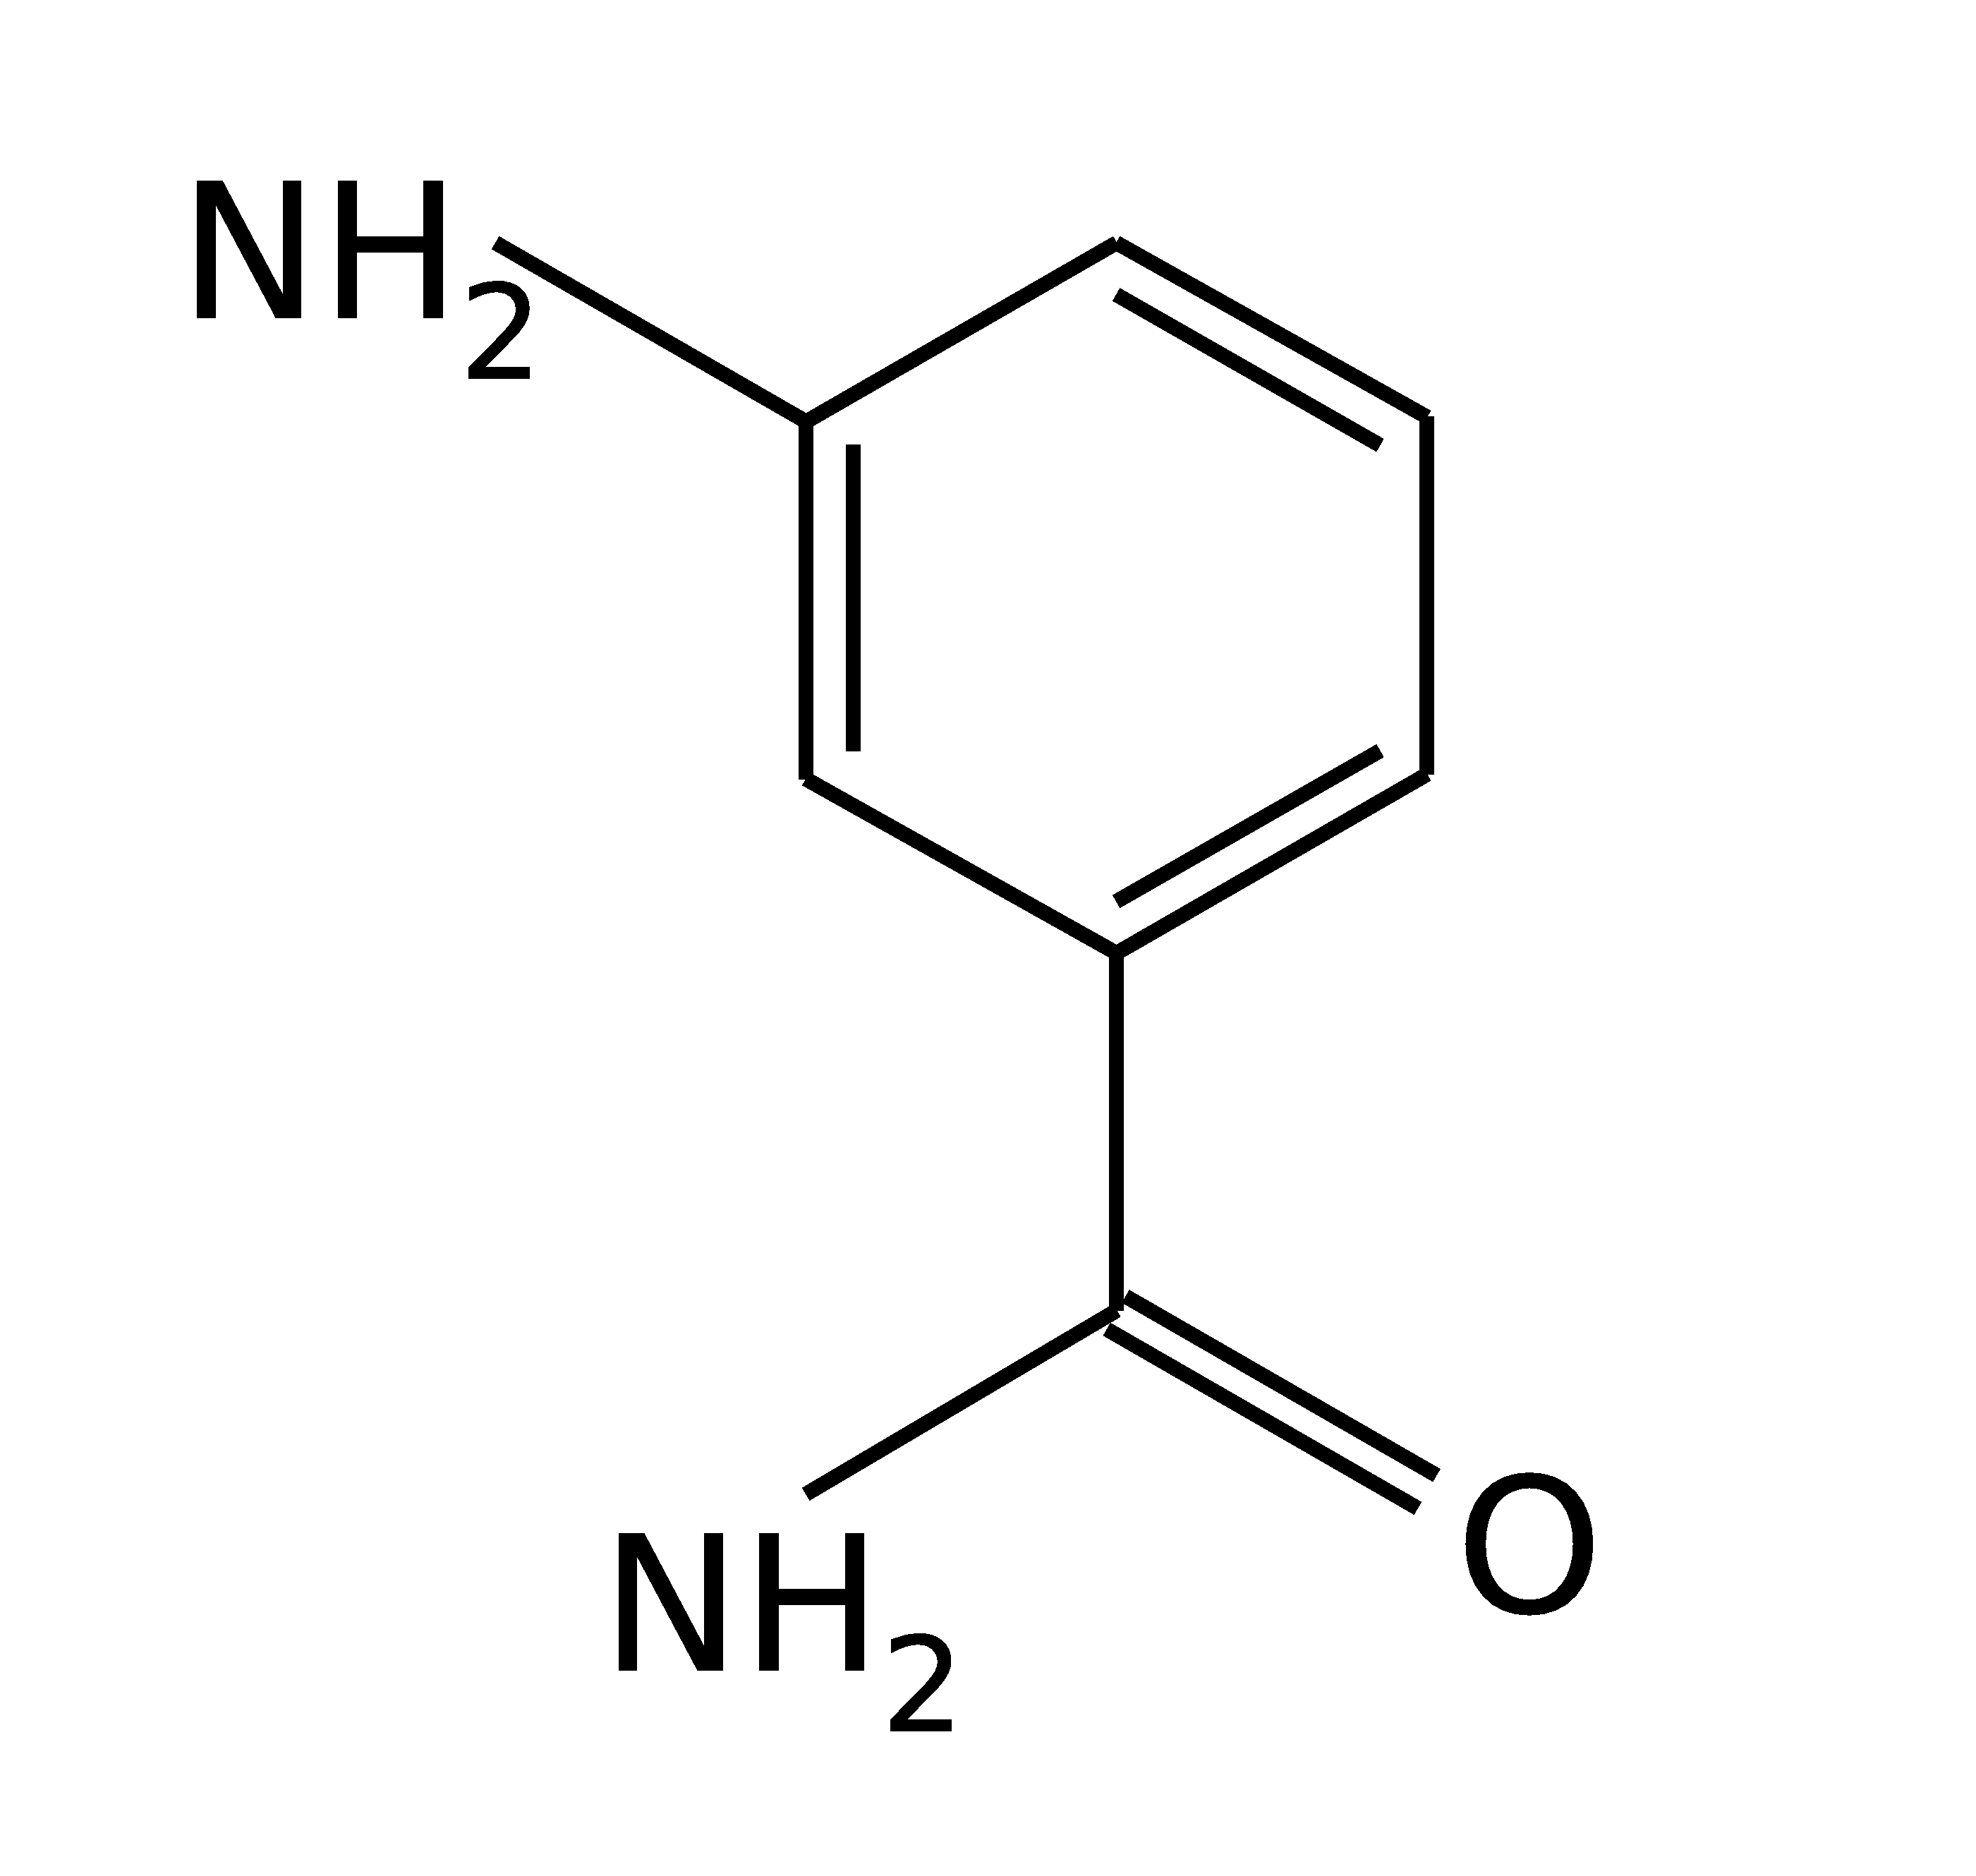
\includegraphics[width=30mm]{3-amino-benzamide-2.png}
    \epsfxsize 30mm
    \epsffile{3-amino-benzamide-2.eps}
    \caption{3-amino-benzamide}{}
    \label{fig:3-amino-benzamide}
  \end{center}
\end{figure}

\begin{trivlist}
\item  How do we make a 3D model of this ligand?

\textsf{We use a SMILES string (and LIBCHECK)\footnote{Alternatively use the Ligand Builder in Coot (\textsf{Calculate $\rightarrow$ Ligand Builder}) which will use PRODRG for restraint generation or even JLigand}.}
\end{trivlist}


\begin{trivlist}
\item So what is the SMILES string for 3-aminobenzamide?
\end{trivlist}

 %% [Draw out the SMILES string].
 %%  NC(=O)c1cccc(N)c1

 If you can't draw out the SMILES string, try this link in your browser:

\texttt{ http://www.molinspiration.com/cgi-bin/properties}
\begin{trivlist}
\item  draw the molecule there and hit the ``Calculate Properties'' button - the
 next pages gives you the SMILES string.

\end{trivlist}

We need to convert this SMILES string representation to a molecule.
In Coot we do that using \textsf{File $\rightarrow$ SMILES...}
\footnote{ Note that the first line is the three letter code,
  conventionally this is 3 uppercase letters, e.g. \texttt{LIG, DRG,
    XXX}.  Note that if you use several different SMILES strings, they
  each should have a different 3-letter-code.} Enter you SMILES string
in the second of the two entry boxes. Press "Go".

\textsl{ After a few moments (in which Coot runs LIBCHECK) a molecule
  will appear at the centre of the screen.}

 \begin{trivlist}
 \item Is it the molecule that you wanted?  

 \textsf{Note: check the hydrogens and planarity.}
 \end{trivlist}


\section{Fitting Ligands}

We how the correct ligand now, So let's move on to search the map for
entities of this kind.

 \textsf{Calculate $\rightarrow$ Other Modelling Tools $\rightarrow$ Find Ligands...}

 We have 2 maps from which to choose.  For now, let's choose the
 2mFo-DFc map and find density clusters above 1.0 sigma.  Make sure
 that you select the correct map and protein molecule and have
 selected the ligand that you made with the SMILES string.

 Press \textsf{"Find 'Em!"}

 \begin{trivlist}
 \item What do you see!? 

\textsf{You should see 4 hits.  }
 \end{trivlist}




Let's use the Fitted Ligands dialog to navigate to these hits.

\begin{trivlist}
\item Do we like all the hits?  If not, why not?  

\textsf{Let's worry about any problematic fittings later on and for
 now, let's concentrate on the nicely fitting solutions.}
\end{trivlist}


\begin{trivlist}
\item If you like the any of the hits, merge them into the main
  protein molecule.

Using \textsf{Calculate $\rightarrow$ Merge Molecules}, 

\end{trivlist}

 In the top pane, select the ligand hits that fit nicely by ticking
 them.  In the lower option menu, select the protein model.  Then
 click "Merge".  Now we have 2 representations of the ligands, which
 can be confusing, so let's use the Display Manager to undisplay the
 Fitted Ligands that we merged into the main protein.

 Using the Fitted Ligand dialog, navigate to the newly added monomers
 and optimise the fit to density - we'll use Real Space Refinement to
 do that.  Use the blue target on right-hand toolbar and click an atom
 in the residue twice.  Do you like the result of the refinement?
 What is the torsion angle of the carboxy-amine?

\section{Presentation}

 We can emphasise the atom positions using 
 \textsf{Extensions $\rightarrow$ Representations $\rightarrow$ Hilight Interesting Site}.

 \begin{trivlist}
 \item Nice?

 \textsf{Maybe\ldots}
 \end{trivlist}

\section{Problem Areas}

OK, now we have fitted the nicely fitting ligands, let's go back to
the problematic blobs.

 \textsf{Validate $\rightarrow$ Find unmodelled blobs}

 We shall search the 2mFo-DFc as did previously using the same protein
 model (which now has the 3-aminobenzamide fitted).  Press "Find
 blobs" \footnote{we could also use \textsf{Validate $\rightarrow$
     Difference Map Peaks} to navigate to these positions.}

\textsl{ We should get a dialog with two blobs listed.}
 
Examine those two blobs.  We know that 3-aminobenzamide does not fit
these blobs well.  What else could these blobs be?  Let's look at the
crystallization and freezing conditions?  Any clues?

 Now, we don't necessarily know the 3-letter-codes of the molecules
 that might fit these blobs. We can use the searching tool in Coot to
 convert between a molecule name and its 3-letter-code.  

 \textsf{File $\rightarrow$ Search Monomer Library\ldots}
 add the molecule name to the entry box and press "Search"

 You will see a list of molecule that include the text you typed as
 part of the molecule names.

 If you click on any of those buttons, Coot runs LIBCHECK and
 generates a molecule and puts it at the centre of the screen.

 You can do this for the 3 or 4 different molecules that you think
 this blob might be.

 The centre of the screen is a bit crowded now.  Undisplay those new
 ligands.  To easily identify the best fitting ligand at the site,
 let's do ligand fitting here.

 \textsf{Calculate $\rightarrow$ Other Modelling Tools $\rightarrow$
   Find Ligands }

 Select the 2mFo-DFc map as usual, and the main protein as before and
 the ligands to search for are the 3 or 4 newly created ligands.

 This time we will Search "Right Here".  You can turn on flexible
 ligands if you like, but this will slow down the search
 considerably. 

\section{Tidying Up}

Real Space refinement is the tool to tidy things up. Using the blue
circle icon on the right, then click click on an atom in the residue
\footnote{or (quicker) simply press the "R" key (if you have the key
  bindings set up).}.

 When we are happy with our fit, we can merge this new ligand into the
 main protein ligand as we did before.

\section{NCS Ligands}

 You may have noticed by now that there are 2 protein chains related
 by non-crystallographic symmetry.  We can exploit this NCS to help
 fit ligands.  We have fitting a ligand that bound to the "A" chain,
 now let's use NCS to position a ligand in related position in the "B"
 chain of the protein.

 \textsf{Extensions $\rightarrow$ NCS $\rightarrow$ NCS Ligands...}

 The protein with the NCS is the main protein as usual, the molecule
 containing the ligand is also the main protein as usual (if we have
 done the merge mentioned above).  We need to know the chain ID of the
 ligand that we have fitted into the "A" chain, to do that double
 left-click an an atom in the ligand. In the graphics you will see
 something like: \texttt{" C1 /1 XXX/E"} - so the chain-id is
 \texttt{"E"}. Also the status bar at the bottom shows information about
 the clicked atom.

 So enter that chain-id in the "Molecule containing ligand" "Chain ID"
 entry.  Then \textsf{"Find Candidate positions"}.
 
 A fitted ligands dialog box pops up and you can use the buttons in
 that dialog to navigate to the NCS ligand positions.

 Refine this NCS ligand position if needed and merge it into the main
 molecule.

\section{For the Adventurous}

If you are feeling adventurous, you can run refmac: \textsf{Calculate
  $\rightarrow$ Model/Fit/Refine $\rightarrow$ Run Refmac...}

 Choose an MTZ file for Refmac and use the file selector to choose the
 same MTZ file that we used in the beginning.

 Examine the resulting molecule.  Are there any problems left to fix?

\section{An SGC Example}

Fit R78 in 5c8g.

\end{document}
